% ======================================================================
%  SIMC 2026  ---  SUBMISSION REPORT  (Endeavour Track)
%  Full worked solutions to Questions 1-3, within the 10-page cap.
%  Format: 12pt Times New Roman (newtx), single spacing, A4, no cover page.
%  Official filename before upload:  SIMC<ID>_<schoolAbbr>.pdf
%  Team: K. Vishnu Kumar . Adithya Kesan Jayakanth . Adithya Anand
%  Compile: pdflatex (run twice).  Figures in doc/FINAL/figs/.
% ======================================================================
\documentclass[12pt,a4paper]{article}

\usepackage[a4paper, margin=1.5cm, headheight=14pt, headsep=9pt, footskip=14pt]{geometry}
\usepackage{amsmath,amsthm}
\usepackage{newtxtext,newtxmath}   % Times New Roman text + matching Times math
\usepackage{bm}
\usepackage{graphicx}
\usepackage{booktabs,array}
\usepackage{xcolor}
\usepackage{titlesec}
\usepackage{fancyhdr}
\usepackage{enumitem}
\usepackage{caption}
\usepackage{listings}
\usepackage{microtype}
\usepackage[hidelinks]{hyperref}

\graphicspath{{figs/}}

\linespread{1.0}
\setlength{\parindent}{1.2em}
\setlength{\parskip}{0.5pt}

\titlespacing*{\section}{0pt}{0.65\baselineskip}{0.2\baselineskip}
\titlespacing*{\subsection}{0pt}{0.4\baselineskip}{0.1\baselineskip}
\titleformat{\section}{\large\bfseries}{\thesection}{0.6em}{}
\titleformat{\subsection}{\normalsize\bfseries}{\thesubsection}{0.6em}{}

\pagestyle{fancy}\fancyhf{}
\fancyhead[L]{\footnotesize\itshape High-Dimensional Data: A Linear-Algebra Account}
\fancyhead[R]{\footnotesize \thepage}
\fancyfoot[C]{\footnotesize SIMC 2026 \,$\cdot$\, Endeavour Track \,$\cdot$\, Team SIMC10}
\renewcommand{\headrulewidth}{0.4pt}

\captionsetup{font=small, labelfont=bf, skip=3pt}

\theoremstyle{definition}
\newtheorem*{claimx}{Claim}

\usepackage[most]{tcolorbox}
\newtcolorbox{callout}[1]{enhanced, colback=blue!4!white, colframe=blue!55!black,
  boxrule=0.5pt, arc=2pt, left=6pt, right=6pt, top=3pt, bottom=3pt,
  fonttitle=\bfseries\footnotesize, fontupper=\small, coltitle=white,
  colbacktitle=blue!55!black, title=#1, before skip=5pt, after skip=5pt}

\DeclareMathOperator{\tr}{tr}
\newcommand{\T}{^{\!\top}}
\newcommand{\norm}[1]{\lVert #1 \rVert}
\newcommand{\R}{\mathbb{R}}
\newcommand{\M}{\mathbb{M}}
\newcommand{\Xt}{\widetilde{\mathbf X}}
\newcommand{\xtv}{\widetilde{\mathbf x}}
\newcommand{\Nt}{\widetilde{N}}

% compact code style
\definecolor{cbg}{gray}{0.965}\definecolor{ccm}{rgb}{0.32,0.46,0.32}\definecolor{ckw}{rgb}{0.10,0.10,0.55}
\lstdefinestyle{py}{language=Python, basicstyle=\ttfamily\footnotesize, backgroundcolor=\color{cbg},
  commentstyle=\color{ccm}\itshape, keywordstyle=\color{ckw}, showstringspaces=false, breaklines=true,
  columns=fullflexible, frame=leftline, framesep=5pt, rulecolor=\color{gray!45}, aboveskip=4pt, belowskip=3pt,
  xleftmargin=8pt}
\lstset{style=py}

\begin{document}

% ----------------------------------------------------------------------
\begin{center}
{\large\bfseries A Linear-Algebra Guide to the Strange Life of High-Dimensional Data}\\[2pt]
{\small Solutions to Questions 1--3 \,\textbullet\, SIMC 2026 Endeavour Challenge \,\textbullet\, 27 May 2026}\\[1pt]
{\small K.\ Vishnu Kumar \quad Adithya Kesan Jayakanth \quad Adithya Anand \,$\cdot$\, PSBB KKN \,$\cdot$\, Team ID SIMC10}
\end{center}
\vspace{-3pt}\noindent\rule{\linewidth}{0.4pt}

% ======================================================================
\section{Markov matrices and the fate of a population}

We are given two organism types whose fractional populations $p_1(t),p_2(t)$ evolve in discrete
generations by $\bm P(t{+}1)=\M\,\bm P(t)$, where
\begin{equation}
  \bm P(t)=\begin{pmatrix}p_1(t)\\ p_2(t)\end{pmatrix},\qquad
  \M=\begin{pmatrix}1-\varepsilon & 0\\[1pt] \varepsilon & 1\end{pmatrix},\qquad \varepsilon\in(0,1).
\end{equation}
Each step, a fraction $\varepsilon$ of type~1 converts to type~2 and nothing returns. The two
component equations are $p_1(t{+}1)=(1-\varepsilon)p_1(t)$ and $p_2(t{+}1)=\varepsilon\,p_1(t)+p_2(t)$.

\subsection{(a) The total population is conserved}
Let $S(t)=p_1(t)+p_2(t)$. Adding the two update equations, the $\varepsilon$ terms cancel:
\begin{equation}
  S(t{+}1)=(1-\varepsilon)p_1(t)+\varepsilon\,p_1(t)+p_2(t)=p_1(t)+p_2(t)=S(t).
\end{equation}
So $S$ never changes, and $S(t)=S(0)$ for all $t$: the total population is conserved.

\subsection{(b) Eigenvalues and eigenvectors}
Because $\M$ is lower triangular its eigenvalues are its diagonal entries, which we confirm from
\begin{equation}
  \det(\M-\lambda\mathbf I)=\det\!\begin{pmatrix}1-\varepsilon-\lambda & 0\\[1pt] \varepsilon & 1-\lambda\end{pmatrix}
  =(1-\varepsilon-\lambda)(1-\lambda)=0
  \;\Longrightarrow\; \lambda_1=1,\ \ \lambda_2=1-\varepsilon .
\end{equation}
The eigenvectors come from solving $(\M-\lambda_i\mathbf I)\bm\nu_i=\bm 0$. For $\lambda_1=1$,
\begin{equation}
  \M-\mathbf I=\begin{pmatrix}-\varepsilon & 0\\[1pt] \varepsilon & 0\end{pmatrix},\qquad
  \begin{pmatrix}-\varepsilon & 0\\[1pt] \varepsilon & 0\end{pmatrix}\!\begin{pmatrix}x\\ y\end{pmatrix}=\bm 0
  \;\Rightarrow\; -\varepsilon x=0 \;\Rightarrow\; x=0\ (y\text{ free}),
\end{equation}
so $\bm\nu_1=(0,1)\T$. For $\lambda_2=1-\varepsilon$,
\begin{equation}
  \M-(1-\varepsilon)\mathbf I=\begin{pmatrix}0 & 0\\[1pt] \varepsilon & \varepsilon\end{pmatrix},\qquad
  \varepsilon x+\varepsilon y=0 \;\Rightarrow\; x+y=0,
\end{equation}
so $\bm\nu_2=(1,-1)\T$. The first eigenvector is the all-type-2 state that the dynamics never
leaves; the second is the transient direction along which type~1 decays.

\subsection{(c) Writing the initial state in the eigenbasis}
With $\bm P(0)=c_1\bm\nu_1+c_2\bm\nu_2=(c_2,\;c_1-c_2)\T$, matching components gives
$c_2=p_1(0)$ and $c_1=p_2(0)+p_1(0)=S(0)$. So $c_1$ is exactly the conserved total from part~(a),
which is a useful consistency check rather than a coincidence. Taking the natural normalisation
$p_1(0)+p_2(0)=1$ with $p_1(0)=\tfrac12$ gives the tidy decomposition
$\bm P(0)=\bm\nu_1+\tfrac12\bm\nu_2$. We give the general coefficients first so that this
normalisation assumption is stated explicitly.

\subsection{(d) Closed-form evolution}
The eigenbasis turns repeated matrix multiplication into ordinary powers. Applying $\M$ once,
\begin{equation}
  \M\bm P(0)=\M(c_1\bm\nu_1+c_2\bm\nu_2)=c_1\M\bm\nu_1+c_2\M\bm\nu_2=c_1\lambda_1\bm\nu_1+c_2\lambda_2\bm\nu_2,
\end{equation}
since $\M\bm\nu_i=\lambda_i\bm\nu_i$. Each further step multiplies mode $i$ by another $\lambda_i$,
so $\M^{t}\bm\nu_i=\lambda_i^{t}\bm\nu_i$ and
\begin{equation}
  \bm P(t)=\M^{t}\bm P(0)=c_1\lambda_1^{t}\bm\nu_1+c_2\lambda_2^{t}\bm\nu_2
  =c_1\,\bm\nu_1+c_2\,(1-\varepsilon)^{t}\,\bm\nu_2 ,
\end{equation}
using $\lambda_1=1$ and $\lambda_2=1-\varepsilon$. Each mode evolves on its own, scaled by its
eigenvalue raised to the power $t$.

\subsection{(e) Long-run behaviour}
\emph{(i) The limit.} Because $0<\varepsilon<1$ we have $0<1-\varepsilon<1$, so
$(1-\varepsilon)^{t}\to0$ as $t\to\infty$. The transient term in~(d) therefore vanishes and
\begin{equation}
  \bm P(t)\;\longrightarrow\;c_1\bm\nu_1=\bigl(0,\;p_1(0)+p_2(0)\bigr)\T ,
\end{equation}
the eigenvector with the larger eigenvalue $\lambda_1=1$; all mass ends up as type~2.

\emph{(ii) Why the structure forces this.} The second column of $\M$ is $(0,1)\T$, so type~2 is
absorbing: once an individual is type~2 it never leaves. Type~1, meanwhile, loses a fraction
$\varepsilon$ every step and is never replenished, so it drains away completely. The eigenvalue
$\lambda_1=1$ carries the surviving steady state and $\lambda_2=1-\varepsilon<1$ governs how
quickly the rest drains into it.

\subsection{(f) Checking (d) and (e) numerically}
We verified the closed form against a direct simulation that uses no analytical input: iterate
$\bm P(t{+}1)=\M\bm P(t)$ for $T=100$ generations at $\varepsilon=0.1$, and compare with the
formula from~(d). The two agree to the last bit of double precision, with maximum discrepancy of
order $10^{-16}$, and the trajectory settles on $(0,1)$ as predicted. The assertion is what makes
this a test rather than a demonstration: if a later edit broke the formula, the cell would stop
rather than quietly plot the wrong thing.
\begin{lstlisting}
P = np.zeros((T+1, 2)); P[0] = p0                  # track A: brute-force iteration
for s in range(T): P[s+1] = M @ P[s]
P_closed = c1*v1 + c2*((1-eps)**t)[:,None]*v2       # track B: closed form from (d)
assert np.max(np.abs(P - P_closed)) < 1e-10         # must agree to machine precision
\end{lstlisting}
Figure~\ref{fig:t1f} shows the result. On the linear axis both populations move monotonically to
their limits; on the semi-logarithmic axis the numeric $p_1(t)$ falls exactly along the line
$\tfrac12(1-\varepsilon)^{t}$, and a straight line there is the signature of geometric decay at
rate $1-\varepsilon$.

\begin{figure}[htbp]\centering
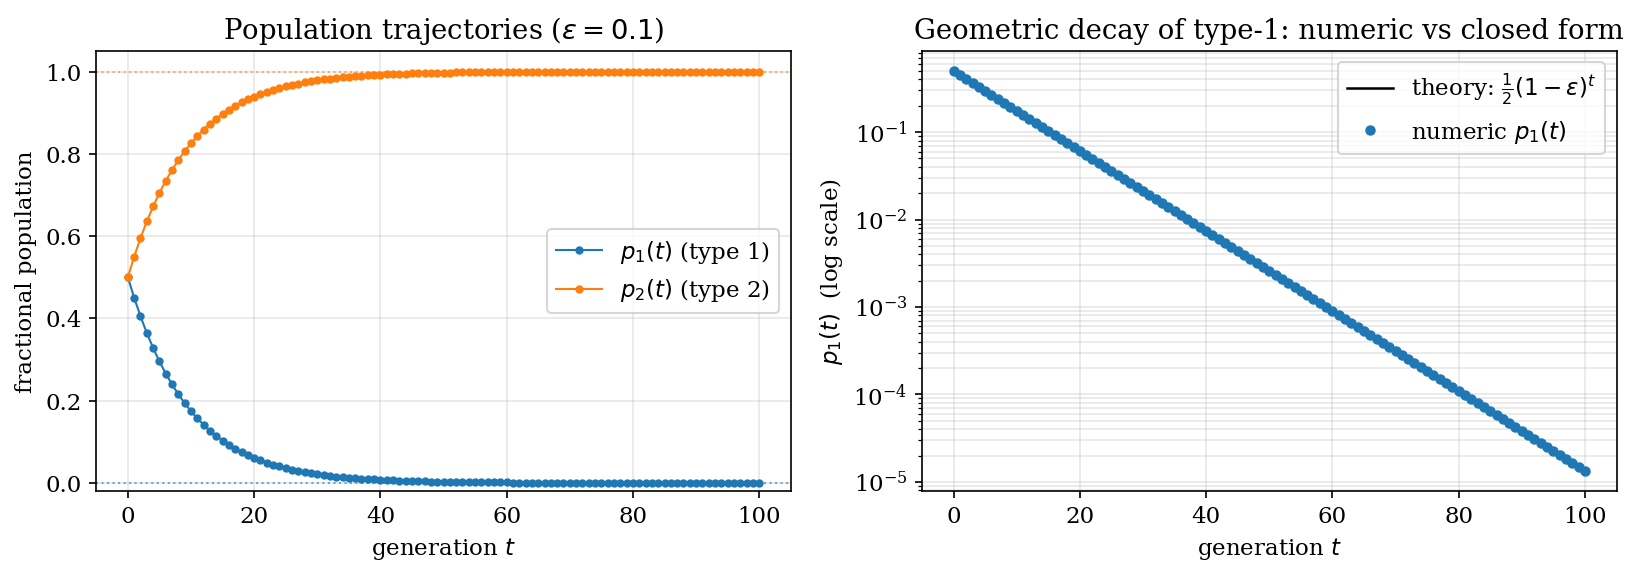
\includegraphics[width=0.66\linewidth]{task1f_trajectories.png}
\caption{Constant $\varepsilon=0.1$. Left: $p_1,p_2$ converge to $(0,1)$. Right: the simulated
$p_1(t)$ (markers) sits on the closed form $\tfrac12(1-\varepsilon)^t$ (line) on a log axis,
confirming both the formula of~(d) and the geometric rate.}\label{fig:t1f}
\end{figure}

\subsection{(g) A conversion rate that fades over time}
Now let the rate decay, $\varepsilon(t)=\varepsilon_0 e^{-t/t_0}$, so the update matrix
$\M(t)$ is different at every step. The key observation is that the eigenvectors do not depend on
$\varepsilon$, so $\bm\nu_1$ and $\bm\nu_2$ are shared by every $\M(t)$:
$\M(t)\bm\nu_1=\bm\nu_1$ and $\M(t)\bm\nu_2=(1-\varepsilon(t))\bm\nu_2$. The state is the ordered
product $\bm P(t)=\M(t{-}1)\cdots\M(0)\,\bm P(0)$. Acting on $\bm P(0)=c_1\bm\nu_1+c_2\bm\nu_2$,
the persistent mode is multiplied by $1$ at every step, while the transient mode picks up one
factor $1-\varepsilon(s)$ at step $s$; after $t$ steps these factors have accumulated into a
product:
\begin{equation}
  \bm P(t)=c_1\bm\nu_1+c_2\Bigl[\textstyle\prod_{s=0}^{t-1}\bigl(1-\varepsilon_0e^{-s/t_0}\bigr)\Bigr]\bm\nu_2 .
\end{equation}
So the geometric power $(1-\varepsilon)^{t}$ of part~(d) becomes a \emph{product}
$\prod_{s}(1-\varepsilon(s))$; the power $(1-\varepsilon(t))^{t}$ would be correct only if the
matrix were fixed.

This product behaves very differently from the constant-rate case, which is the interesting part.
With $\varepsilon$ fixed, every factor is the same number below $1$, so the product shrinks all the
way to $0$ and type~1 disappears. With a \emph{fading} rate the factors $1-\varepsilon(s)$ climb
back towards $1$ as $\varepsilon(s)\to0$, and they reach $1$ fast enough that the running product
stops changing and settles at a strictly positive value $\Pi_\infty$ instead of $0$ -- once we are
multiplying by numbers indistinguishable from $1$, the product barely moves. The conversion has
effectively switched off, freezing a residue $c_2\Pi_\infty$ in the $\bm\nu_2$ direction, so the
population settles at $\bm P(\infty)=c_1\bm\nu_1+c_2\Pi_\infty\bm\nu_2$ and type~1 is \emph{never
fully depleted}. A fading conversion rate therefore traps a small permanent population of type~1,
the qualitative correction to parts~(d)--(e).

\subsection{(h) Checking the fading rate}
We validated the product formula exactly as in~(f), iterating with a freshly built $\M(s)$ at each
step ($\varepsilon_0=0.5$, $t_0=10$) and comparing against the closed form; agreement is again at
the $10^{-16}$ level. Figure~\ref{fig:t1h} overlays the fading-rate trajectory on the constant-rate
case. The contrast is the whole point: with constant $\varepsilon$, $p_1$ heads for zero in a
straight log-line, whereas with $\varepsilon(t)$ it bends and locks onto a positive plateau once
the rate has effectively vanished. The measured residue matches the small-rate estimate
$\tfrac12 e^{-\varepsilon_0 t_0}$ to the expected accuracy.

\begin{figure}[htbp]\centering
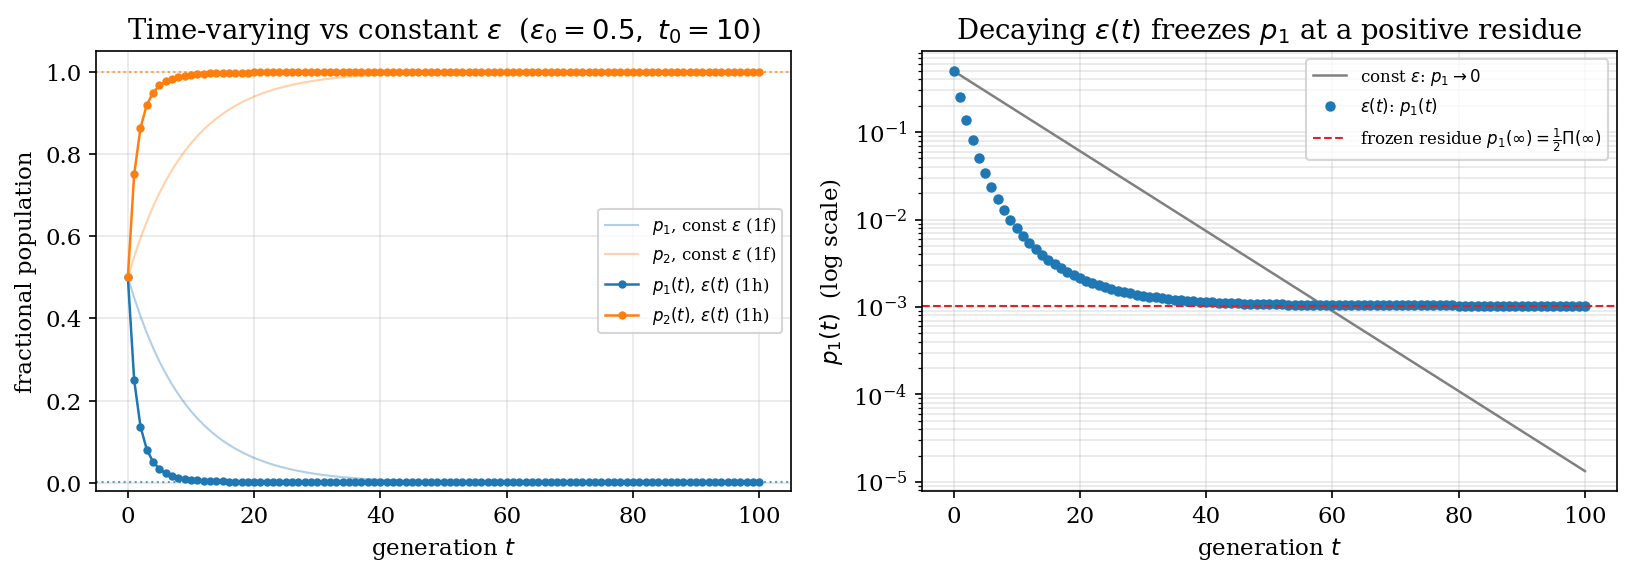
\includegraphics[width=0.66\linewidth]{task1h_trajectories.png}
\caption{Fading rate $\varepsilon(t)=\varepsilon_0 e^{-t/t_0}$ (solid) against constant
$\varepsilon$ (faded). Right panel, log axis: the constant case drains to zero, while the fading
case freezes at the positive residue $c_2\Pi_\infty$ (dashed).}\label{fig:t1h}
\end{figure}

% ======================================================================
\section{The power method and the singular value decomposition}

Here $\mathbf X$ is a symmetric $n\times n$ matrix with eigenvalues
$|\lambda_1|>|\lambda_2|\ge\cdots\ge|\lambda_n|$ and an orthonormal eigenbasis
$\bm\nu_1,\dots,\bm\nu_n$. The power method starts from a unit vector and repeats
$\bm x_{k+1}=\mathbf X\bm x_k/\norm{\mathbf X\bm x_k}$.

\subsection{(a) Why the iteration finds the dominant eigenvector}
\begin{claimx} If $\bm x_0$ has a nonzero component along $\bm\nu_1$, then $\bm x_k\to\pm\bm\nu_1$. \end{claimx}
Normalisation only rescales, so $\bm x_k$ points the same way as $\bm y_k=\mathbf X^{k}\bm x_0$.
Expand $\bm x_0=\sum_i a_i\bm\nu_i$ with $a_1\neq0$. Since $\mathbf X^{k}\bm\nu_i=\lambda_i^{k}\bm\nu_i$,
\begin{equation}
  \bm y_k=a_1\lambda_1^{k}\bm\nu_1+\sum_{i\ge2}a_i\lambda_i^{k}\bm\nu_i .
\end{equation}
Measuring the off-axis part relative to the leading term, and using orthonormality,
\begin{equation}
  \rho_k=\frac{\bigl\lVert\sum_{i\ge2}a_i\lambda_i^{k}\bm\nu_i\bigr\rVert}{|a_1|\,|\lambda_1|^{k}}
  =\frac{1}{|a_1|}\sqrt{\sum_{i\ge2}a_i^{2}\Bigl(\tfrac{\lambda_i}{\lambda_1}\Bigr)^{2k}} .
\end{equation}
Every ratio $|\lambda_i/\lambda_1|<1$, so each term vanishes and $\rho_k\to0$: the iterate aligns
with $\bm\nu_1$, and after normalising, $\bm x_k\to\pm\bm\nu_1$, with the sign tracking
$\operatorname{sign}(a_1\lambda_1^{k})$.

\subsection{(b) Rate of convergence and the spectral gap}
The same expression bounds how fast this happens. Writing $\omega_i=a_i^{2}\lambda_i^{2k}\ge0$,
\begin{equation}
  \frac{\rho_{k+1}}{\rho_k}=\frac{1}{|\lambda_1|}\sqrt{\frac{\sum_{i\ge2}\omega_i\lambda_i^{2}}{\sum_{i\ge2}\omega_i}}
  \le\frac{1}{|\lambda_1|}\sqrt{\lambda_2^{2}}=\Bigl|\tfrac{\lambda_2}{\lambda_1}\Bigr|<1,
\end{equation}
because the fraction under the root is a weighted average of the $\lambda_i^{2}$ ($i\ge2$), which
cannot exceed the largest, $\lambda_2^{2}$. Convergence is therefore geometric at rate
$|\lambda_2/\lambda_1|$. The quantity that controls everything is the spectral gap between the two
largest eigenvalues: a wide gap means fast, stable convergence, a narrow one means slow and
fragile.

\subsection{(c) When the gap closes}
Take $\mathbf X=\operatorname{diag}(1,-1)$, so $|\lambda_1|=|\lambda_2|=1$ and there is no gap. For
a generic start $(a,b)$ one finds $\mathbf X^{k}(a,b)\T=(a,(-1)^{k}b)\T$. The norm is preserved, so
after normalisation the iterate flips forever between $(a,b)$ and $(a,-b)$ and never settles. This
is not merely slow convergence but a structural failure. The power method works by amplifying each
eigencomponent by its own factor $\lambda_i^{k}$, and the top one wins only because it is strictly
largest. When two leading eigenvalues share a magnitude, their relative weights never change and
there is no mechanism to select one: the iterate keeps whatever mixture it began with, oscillating
when the signs differ or, if $\lambda_1=\lambda_2$, drifting to an arbitrary vector of the shared
eigenspace. The near-degenerate case is worse in practice than in theory. The iteration count
scales like $1/(1-|\lambda_2/\lambda_1|)$ and blows up, while the useful per-step separation
between $\bm\nu_1$ and $\bm\nu_2$ shrinks to the level of the $10^{-16}$ rounding error that every
floating-point step injects, at which point the computed ordering of the two eigenvalues becomes
ambiguous.

\subsection{(d) The matrices $\mathbf X\T\mathbf X$ and $\mathbf X\mathbf X\T$}
Let $\mathbf X$ now be a general $m\times n$ matrix. Both products are symmetric, since
$(\mathbf X\T\mathbf X)\T=\mathbf X\T\mathbf X$ and likewise for $\mathbf X\mathbf X\T$, and both
are positive semi-definite, because for any $\bm w$,
\begin{equation}
  \bm w\T(\mathbf X\T\mathbf X)\bm w=\norm{\mathbf X\bm w}^{2}\ge0,\qquad
  \bm w\T(\mathbf X\mathbf X\T)\bm w=\norm{\mathbf X\T\bm w}^{2}\ge0 .
\end{equation}
Being symmetric and positive
semi-definite, each has real non-negative eigenvalues, so $\sigma_i=\sqrt{\lambda_i}$ is well
defined. They also share their nonzero eigenvalues. If $\mathbf X\T\mathbf X\bm v=\lambda\bm v$
with $\lambda\neq0$, then left-multiplying by $\mathbf X$,
\begin{equation}
  (\mathbf X\mathbf X\T)(\mathbf X\bm v)=\lambda(\mathbf X\bm v),
\end{equation}
and $\mathbf X\bm v\neq\bm 0$ (otherwise $\lambda\bm v=\mathbf X\T\mathbf X\bm v=\bm 0$ would force
$\lambda=0$). So $\mathbf X\bm v$ is an eigenvector of $\mathbf X\mathbf X\T$ with the same
eigenvalue, and the symmetric argument gives the converse. The shared nonzero values are the
$\sigma_i^{2}$. This is the fact Question~3 leans on to connect its covariance and Gram analyses.

\subsection{(e) A power-method SVD, and a worked example}
To find the leading singular triplet of an $N\times M$ matrix $\mathbf X$, run the power method on
whichever of $\mathbf X\T\mathbf X$ ($M\times M$) or $\mathbf X\mathbf X\T$ ($N\times N$) is
smaller, since both square to size $\min(N,M)$ and share the spectrum of interest. Recover the top
eigenvector $\bm v_1$, set $\sigma_1=\sqrt{\bm v_1\T(\mathbf X\T\mathbf X)\bm v_1}$ from the
Rayleigh quotient, and obtain the partner vector by a single multiplication,
$\bm u_1=\mathbf X\bm v_1/\sigma_1$.

Concretely, take $\mathbf X=\bigl(\begin{smallmatrix}1&0\\0&1\\1&1\end{smallmatrix}\bigr)$ with
$N=3,M=2$. The smaller matrix is
$\mathbf X\T\mathbf X=\bigl(\begin{smallmatrix}2&1\\1&2\end{smallmatrix}\bigr)$, with eigenvalues
$1$ and $3$. The dominant one gives $\lambda_1=3$, $\sigma_1=\sqrt3$, and
$\bm v_1=\tfrac1{\sqrt2}(1,1)\T$. Then
$\bm u_1=\mathbf X\bm v_1/\sigma_1=\tfrac1{\sqrt6}(1,1,2)\T$. Both defining relations hold:
$\mathbf X\bm v_1=\tfrac1{\sqrt2}(1,1,2)\T=\sigma_1\bm u_1$, and
$\mathbf X\T\bm u_1=\tfrac{3}{\sqrt6}(1,1)\T=\sigma_1\bm v_1$, confirming the triplet by hand.

% ======================================================================
\section{Cleaning, principal components, and clustering of spectra}

The third question hands us \texttt{mystery\_matrix1.npy}, a collection of infrared absorbance
spectra. We treat it as a design matrix $\mathbf X\in\R^{N\times M}$ with rows indexing samples
(vials) and columns indexing features (frequency channels), so $\mathbf X_{ij}$ is the absorbance
of vial $i$ at frequency $j$.

\subsection{(a) Orienting and cleaning the matrix}
The file loads as a $3401\times1000$ array. Two things are worth saying before any analysis. First,
the array is stored transposed relative to the row-as-sample convention, so we transpose once so
that rows are samples. Second, the prompt quotes $M=3041$ features whereas the file has $3401$
columns, a digit transposition; we use the array's true dimension and key off the axis of length
$1000$ rather than hard-coding either number.

An empty vial records only background noise, which is small and flat, so it has a small Euclidean
norm $\norm{\bm x_i}=(\sum_j \mathbf X_{ij}^2)^{1/2}$. Sorting the $1000$ norms makes the structure
plain: $40$ vials cluster near $\norm{\bm x}\approx1.6$, then there is an empty gap, and the bulk
begins near $4.3$. We place the threshold in that gap. Crucially the count of flagged vials does
not move for any cutoff between $2.0$ and $4.0$, which is the evidence that the cut is principled
rather than tuned. This removes exactly $T=40$ empties (rows $960$--$999$). As an independent
check, the removed spectra are $50.2\%$ exact zeros, consistent with background noise clipped at
zero (which is exactly zero with probability about a half), against $24.5\%$ for the genuine
spectra.

A second defect is hiding in the upper tail, one the prompt does not mention. Thirty-six vials sit
near $\norm{\bm x}\approx8.9$ (rows $924$--$959$), separated from the bulk by a gap roughly five
times wider than any gap inside it. We keep a vial only if its norm lies between the two cuts,
implemented as a Boolean mask so the operation is non-destructive and index-preserving, which
leaves $\Nt=924$ spectra. We were initially reluctant to discard a second group on a hunch, so we
tested it: in the top-four principal-component space the $36$ form one tight, isolated cluster, and
removing them lowers the total cluster count by exactly one while leaving every other group
untouched (Figure~\ref{fig:clean}, right). The decision is therefore clean and, because it is a
mask, entirely reversible.

\begin{figure}[htbp]\centering

\includegraphics[height=3.15cm]{q3a_part_i.png}\hfill

\includegraphics[height=3.15cm]{q3a_part_ii_clusters.png}
\caption{Cleaning. Left: the row-norm distribution, with $40$ empty vials below a clean gap
(threshold dashed). Right: the $36$ high-norm vials (red) form a single isolated cluster in the
leading PC plane; removing them deletes exactly one cluster.}\label{fig:clean}
\end{figure}

\subsection{(b) Feature variance and the covariance matrix}
We mean-centre each feature, $\Xt_{ij}=\mathbf X_{ij}-\bar{\mathbf X}_j$, which removes the shared
average spectrum so the analysis describes how samples differ rather than what they have in common.
The covariance matrix is $\mathbf C=\tfrac1\Nt\Xt\T\Xt\in\R^{M\times M}$. Its diagonal entries are
exactly the feature variances, $\mathbf C_{jj}=\tfrac1\Nt\sum_k\Xt_{kj}^2=\mathrm{Var}_j$, since
the columns now have zero mean, and it is symmetric because $(\Xt\T\Xt)\T=\Xt\T\Xt$. The trace is
the total variance, $\tr\mathbf C=\sum_j\mathrm{Var}_j$, and it is invariant under any orthonormal
change of basis, $\tr(\mathbf Q\T\mathbf C\mathbf Q)=\tr(\mathbf C\mathbf Q\mathbf Q\T)=\tr\mathbf C$,
so it also equals $\sum_i\lambda_i$. Numerically $\tr\mathbf C\approx7.90$, and we use the identity
$\sum_i\lambda_i=\tr\mathbf C$ later as a check on the eigendecomposition.

The single most variable feature is $j^\star=910$, with $\mathbf C_{j^\star j^\star}\approx0.0199$.
More telling is the shape of the variance profile (Figure~\ref{fig:var}): it is not spread evenly
across the $3401$ channels but concentrates in a few narrow bands, with broad flat stretches of
baseline in between. The profile itself looks like a spectrum. Those bands are the frequencies
where the dominant molecules absorb and where vials genuinely differ; the flat regions carry almost
no discriminating information. The data is, in other words, highly redundant, which is precisely
the structure principal component analysis exploits next.

\begin{figure}[htbp]\centering

\includegraphics[width=0.56\linewidth]{q3b_variance.png}
\caption{Per-feature variance $\mathbf C_{jj}$ across the $3401$ frequencies, with the maximum at
$j^\star=910$ (dashed). Variance lives in a handful of molecular bands, not the baseline.}\label{fig:var}
\end{figure}

\subsection{(c) The eigenspectrum}
For a unit direction $\bm w$ the variance of the projected data is $\bm w\T\mathbf C\bm w$, and for
an eigenvector this equals the eigenvalue; since $\bm w\T\mathbf C\bm w=\tfrac1\Nt\norm{\Xt\bm w}^2\ge0$,
every $\lambda_i\ge0$. By the spectral theorem $\mathbf C$ has an orthonormal eigenbasis, so we
diagonalise it with \texttt{numpy.linalg.eigh}, the solver for symmetric matrices, which returns
real eigenvalues and orthonormal eigenvectors and is both faster and more stable than the general
\texttt{eig}. We sort the eigenvalues in decreasing order and clip rounding-level negatives to zero.
\begin{lstlisting}
C = (Xc.T @ Xc) / Nt                          # covariance (M x M); Xc is mean-centred X
w, V = np.linalg.eigh(C)                       # symmetric solver: real, orthonormal
order = np.argsort(w)[::-1]
eigvals = np.clip(w[order], 0, None); eigvecs = V[:, order]
kstar = int(np.argmax(eigvals[:30] / eigvals[1:31])) + 1   # elbow = largest consecutive ratio
\end{lstlisting}

The leading eigenvalues are tabulated below. The ratio of the two largest is
$\lambda_1/\lambda_2\approx3.53$, and $\lambda_1$ alone accounts for about $31\%$ of the total
variance, so one direction clearly dominates the variation. A large ratio of this kind is exactly
the wide spectral gap that, by Question~2, would make the power method converge quickly here, and
it signals that the data has strong low-dimensional structure.

\begin{table}[htbp]\centering\small
\begin{tabular}{lccccccccc}
\toprule
$k$ & 1 & 2 & 3 & 4 & 5 & 6 & 7 & 8 & 9\\
$\lambda_k$ & 2.492 & 0.705 & 0.590 & 0.254 & 0.123 & 0.105 & 0.078 & 0.039 & 0.0093\\
\bottomrule
\end{tabular}
\caption{Leading eigenvalues. The drop $\lambda_8/\lambda_9\approx4.1$ is the largest in the
spectrum and marks the elbow.}\label{tab:eig}
\end{table}

To find the number of meaningful components we look for the elbow, the largest multiplicative drop
between consecutive eigenvalues. We use a ratio rather than a difference because the boundary
between signal and noise is multiplicative on the logarithmic scale of Figure~\ref{fig:spectrum}.
The largest drop is $\lambda_8/\lambda_9\approx4.1$, giving $k^\star=8$. On the log plot the first
eight eigenvalues fall steeply and the rest lie on a near-flat noise floor of around $900$ tiny,
slowly-decreasing values. Eight signal components is satisfyingly close to the roughly ten dominant
molecules referred to in part~(h): the spectra are mixtures of a small number of chemical
components, so only a handful of independent directions carry real signal.

\begin{callout}{Intrinsic dimension}
The nominally $3401$-dimensional data has only $k^\star=8$ signal directions. The elbow is set by
the largest multiplicative drop, $\lambda_8/\lambda_9\approx4.1$; everything beyond it lies on a
flat noise floor. Eight signal dimensions echoes the $\sim10$ dominant molecules of part~(h).
\end{callout}

It is tempting to instead keep ``$95\%$ of the variance'', but here that rule is misleading. The
eight signal components explain only about $55\%$ of the variance, and reaching $95\%$ takes $667$
components (Table~\ref{tab:cum}), because the noise floor, though negligible term by term, is
spread over hundreds of dimensions that sum to a large share. A $95\%$ cut would drag in some $660$
noise directions and badly overstate the dimensionality. The elbow is the honest measure.

\begin{table}[htbp]\centering\small
\begin{tabular}{lccccc}
\toprule
cumulative variance & $50\%$ & $80\%$ & $90\%$ & $95\%$ & $99\%$\\
components $k$ & 4 & 309 & 516 & 667 & 850\\
\bottomrule
\end{tabular}
\caption{Components needed to reach each variance threshold. Contrast the eight signal components
(about $55\%$) with the $667$ required for $95\%$.}\label{tab:cum}
\end{table}

\begin{figure}[htbp]\centering

\includegraphics[width=0.66\linewidth]{q3c_spectrum.png}
\caption{Eigenvalue spectrum on linear (left) and logarithmic (right) axes. The log plot shows a
sharp elbow at $k^\star=8$ followed by a flat noise floor.}\label{fig:spectrum}
\end{figure}

A threshold-free reading agrees with the elbow. The explained-variance ratio of component $k$ and
the \emph{participation ratio} (a continuous effective dimension) are
\begin{equation}
  r_k=\frac{\lambda_k}{\sum_j\lambda_j},\qquad
  d_{\mathrm{eff}}=\frac{\bigl(\sum_i\lambda_i\bigr)^2}{\sum_i\lambda_i^{2}} .
\end{equation}
The participation ratio needs no cutoff: it is large when many eigenvalues share the variance and
small when a few dominate. Here $d_{\mathrm{eff}}\approx8.7$, in close agreement with the elbow at
$k^\star=8$ and the $\sim10$ dominant molecules --- three independent criteria (the multiplicative
drop, the participation ratio, and the chemistry) converging on the same handful of dimensions.

\subsection{(d) Reading the leading eigenvector}
The leading eigenvector $\bm\nu_1\in\R^M$ assigns a loading to each frequency, and the scores
$z_i=\xtv_i\cdot\bm\nu_1$ are the one-dimensional summaries of greatest spread. Eigenvectors are
defined only up to sign, so we fix the largest loading positive. The loadings are not spread
evenly: they concentrate on two narrow bands, near $j\approx900$--$960$ and $3150$--$3260$, and
about $27\%$ of the entries are negative. So $\bm\nu_1$ is a contrast direction, measuring the
balance of absorption between bands, not overall brightness. Using cosine similarity, which is
scale-free, $\bm\nu_1$ matches a mean-centred spectrum at about $0.92$ but the raw spectrum at only
$0.67$ and the mean spectrum at $0.03$. Living in the centred space by construction, it is nearly
orthogonal to the shared mean and behaves like a difference spectrum (Figure~\ref{fig:lead}): it
captures how the most distinctive vial departs from the average, which is the chemical contrast
that separates the mixtures most strongly. The echo of Question~1 is hard to miss, where the
dominant eigenvector again carried the structure that survived.

\begin{figure}[htbp]\centering

\includegraphics[width=0.58\linewidth]{q3d_v1_vs_row.png}
\caption{The leading eigenvector $\bm\nu_1$ (green) overlaid on the best-matching centred spectrum
(cosine $\approx0.92$). It reads as a difference spectrum supported on two molecular bands.}\label{fig:lead}
\end{figure}

\subsection{(e) Clusters in covariance space}
Projecting each vial onto the top four eigenvectors gives compressed coordinates
$\mathbf Z=\Xt\mathbf V_4\in\R^{\Nt\times4}$, four scores per vial. The six pairwise scatter plots
(Figure~\ref{fig:cov}) show many tight, well-separated blobs. To count them without reaching for a
library we use leader clustering, starting a new cluster whenever a point is farther than a radius
$r$ from every existing centre.
\begin{lstlisting}
def count_clusters(P, r):                      # numpy-only, no sklearn
    centres = [P[0]]
    for p in P[1:]:
        if np.sqrt(((np.array(centres) - p)**2).sum(1)).min() > r:
            centres.append(p)
    return len(centres)
\end{lstlisting}
The count is $25$, and it is stable for any radius between about six and twelve times the median
nearest-neighbour spacing, so it reflects the data rather than the threshold. Each blob is a set of
vials with nearly identical spectra, that is, one chemical mixture, so the $924$ cleaned vials are
about $25$ recipes, comfortably under the ``fewer than $100$'' mentioned in part~(h). Although the
eigenvectors live in feature space, projecting samples onto them exposes sample-space structure,
because similar spectra receive similar scores.

\begin{figure}[htbp]\centering

\includegraphics[width=0.62\linewidth]{q3e_covariance_scatter.png}
\caption{The six pairwise scatter plots of the top-four covariance scores. Each point is a vial;
the data resolves into about $25$ clusters.}\label{fig:cov}
\end{figure}

\subsection{(f) The same question through the Gram matrix}
The Gram matrix $\mathbf G=\tfrac1\Nt\Xt\Xt\T\in\R^{\Nt\times\Nt}$ lives in sample space, with
$\mathbf G_{ij}$ the similarity between vials $i$ and $j$. Because $\Nt=924\ll M=3401$, the Gram
matrix is only $\Nt\times\Nt$ rather than $M\times M$, so diagonalising it costs $(M/\Nt)^2\approx
13.5$ times less than the covariance route --- exactly the ``use the smaller matrix'' rule of
Question~2(e). By the result of Question~2(d) it shares the nonzero eigenvalues of $\mathbf C$, which
we confirm numerically: the top eight Gram eigenvalues match the top eight covariance eigenvalues to
within $10^{-6}$. A Gram eigenvector's components are
themselves the sample coordinates, with no projection of $\Xt$ needed; scaling by $\sqrt{\Nt\lambda}$
matches the units of part~(e). The six Gram scatter plots reproduce those of the covariance analysis
up to per-axis sign flips, and the same leader-clustering rule again returns $25$ clusters (the two
sets of scores are overlaid explicitly in Figure~\ref{fig:compare} of part~g). Whether we view the
data through its features or through sample-to-sample similarity, the structure is the same.

\subsection{(g) Are the two clusterings really the same?}
They are, and necessarily so. If $\bm\nu$ is an eigenvector of
$\mathbf C=\tfrac1\Nt\Xt\T\Xt$ with eigenvalue $\lambda$, then $\Xt\bm\nu$ is an eigenvector of
$\mathbf G=\tfrac1\Nt\Xt\Xt\T$ with the same $\lambda$, so the two matrices share their nonzero
spectrum. The cleaner statement uses the singular value decomposition. Writing
$\Xt=\mathbf U\Sigma\mathbf V\T$, the covariance and Gram score matrices are
\begin{equation}
  \mathbf Z=\Xt\mathbf V=\mathbf U\Sigma,\qquad
  \mathbf Z_{\mathrm g}=\mathbf U\sqrt{\Nt\lambda}=\mathbf U\Sigma ,
\end{equation}
the \emph{same} matrix $\mathbf U\Sigma$, identical up to the arbitrary sign of each
eigenvector. We checked this directly: the $4\times4$ correlation matrix between the two score sets
is the identity in absolute value, $1$ on the diagonal and $0$ off it, and the coordinates agree in
magnitude to about $10^{-14}$, with the first and fourth axes happening to come out sign-flipped
(Figure~\ref{fig:compare}). Because the two point clouds are the same up to reflecting individual
axes, the clusters and their count must coincide, which is why both routes give $25$.

The two views answer different-sounding questions that turn out to be one question. Covariance space
asks which combination of frequencies a vial expresses; Gram space asks which other vials it
resembles. Both place vials with nearly identical spectra at the same point, so proximity in either
coordinate system means the same chemical mixture.

\begin{figure}[htbp]\centering

\includegraphics[width=0.72\linewidth]{q3g_compare.png}
\caption{Covariance (3e) against Gram (3f). Left: the absolute correlation between the two score
sets, the identity. Right: the six PC-pair scatters with covariance scores (blue circles) and
sign-aligned Gram scores (orange dots) overlaid; they coincide point for point, so the two methods
return the identical $25$ clusters.}\label{fig:compare}
\end{figure}

\subsection{(h) The forgetful taste tester}
The brief: the $1000$ vials hold fewer than $100$ unique fermented-drink samples (one per vial),
fingerprinted by ten dominant molecules whose absorption bands the spectroscopy targets.

\emph{(i) How many unique samples were there?} Our analysis answers this directly: about
\textbf{25}. After discarding the $40$ empty vials and the $36$ corrupted high-norm vials, the $924$
genuine spectra fall into $25$ tight clusters, and each cluster is a set of nearly identical spectra,
that is, one recipe. We trust the figure because it is stable rather than fitted: it holds across
clustering radii spanning a factor of two, and the same $25$ emerges from two independent
constructions, the covariance matrix and the Gram matrix (part~g). It also sits well under the stated
bound of one hundred. The ten dominant molecules surface as the eight signal dimensions of the
eigenspectrum: each spectrum is a non-negative mixture of about ten absorption signatures, so the
mean-centred data needs only that many independent directions, and PCA recovers them as the
$k^\star=8$ components standing above the noise floor. (The $36$ high-norm vials are a measurement
fault, not a $26$th recipe; part~(a) shows they form a single corrupted group.)

The $25$ groups are also near-uniform in size --- $24$ of them hold $37$ replicate vials and one
holds $36$, so $24\times37+36=924$ exactly (Figure~\ref{fig:q3h}). A near-constant replicate count
is the fingerprint of a designed taste test that measured a fixed menu of recipes several dozen
times each, which is exactly what we would expect once the lost labels are restored.

\begin{figure}[htbp]\centering
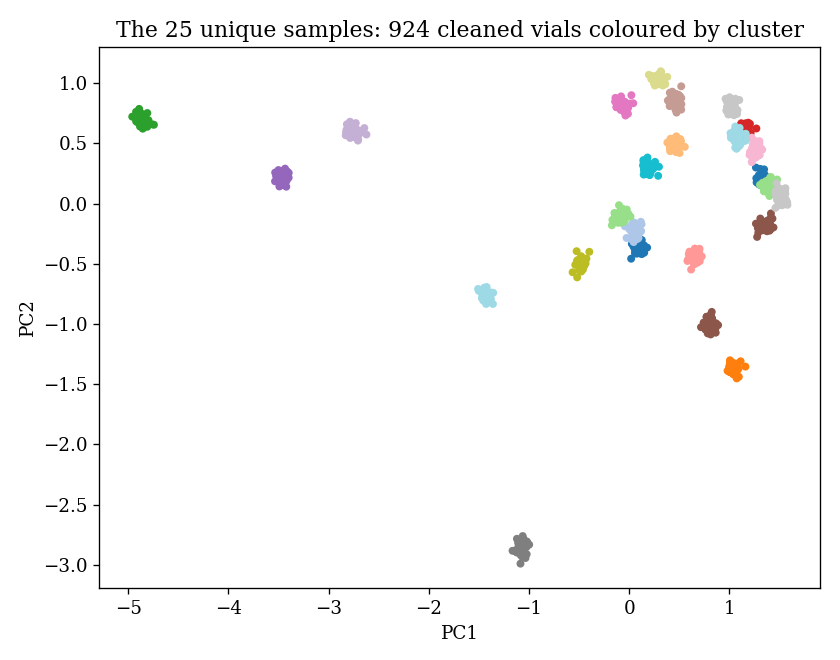
\includegraphics[width=0.46\linewidth]{q3h_clusters.png}
\caption{The $924$ cleaned vials, coloured by cluster, resolve into $25$ well-separated groups in
the leading covariance-score plane. The groups are near-uniform in size ($24\times37+36=924$), the
signature of a designed experiment with $25$ unique samples.}\label{fig:q3h}
\end{figure}

\begin{callout}{Answer to Question 3(h)}
There were about \textbf{$25$ unique food samples}. The $924$ genuine spectra form $25$ tight
clusters of ${\sim}37$ replicate vials each; the count is stable across a factor-of-two range of
clustering radii and is reproduced independently by the covariance and Gram routes (part~g), which
by the Question~2(d) duality is a genuine cross-check rather than a coincidence.
\end{callout}

\emph{(ii) Which earlier parts made this possible?} Almost all of them, which is the real lesson of
the question. The cleaning in~(a) was a precondition, since the empties and especially the outliers
would otherwise have invented spurious clusters and skewed the variance. The mean-centring and
covariance of~(b) and the eigenspectrum of~(c) compressed $3401$ noisy features down to the eight
that carry signal, without which the clusters are invisible to the eye. The projection and clustering
of~(e) produced the count, the Gram route of~(f) reproduced it, and the comparison in~(g) turned that
agreement into a genuine cross-check rather than a coincidence, resting on the
$\mathbf X\T\mathbf X$ / $\mathbf X\mathbf X\T$ duality proved in Question~2(d). Even Question~1
supplies the guiding idea, that the leading eigenvectors of the right matrix carry the structure a
system settles into. Our estimate of $25$ is therefore not one measurement but the consistent reading
of the whole pipeline.

% ======================================================================
\section{Validation, robustness, and limitations}
We tried to make every headline number answerable by more than one route. In Question~1 each closed
form is checked against a direct iteration to the limit of double precision. In Question~3 the trace
identity $\tr\mathbf C=\sum_i\lambda_i\approx7.90$ confirms the eigendecomposition, the Gram and
covariance spectra agree to $10^{-6}$, and the two clusterings agree exactly, which is the empirical
face of the Question~2(d) theorem. The hand-worked SVD example satisfies both defining relations.

The results are stable where it matters. The empty-vial count does not change for any threshold in
$[2.0,4.0]$, and the cluster count holds for clustering radii spanning a factor of two, so neither
headline depends on a tuned parameter. The elbow at $k^\star=8$ rests on a fourfold multiplicative
drop, far clear of the noise floor's near-unit ratios.

The compression is principled rather than ad hoc. By the Eckart--Young theorem, projecting onto the
top $k$ eigenvectors is the \emph{best} rank-$k$ approximation of $\Xt$ in the least-squares sense
--- the same singular value decomposition of Question~2, now read as an approximation rather than a
factorisation, with squared error equal to the sum of the discarded eigenvalues $\sum_{i>k}\lambda_i$.
Keeping $k^\star=8$ replaces each $3401$-number spectrum by $8$ scores, a $425$-fold reduction, while
retaining the $\approx55\%$ of the variance that genuinely separates the mixtures; the discarded
$\approx45\%$ is the noise floor, spread so thinly --- about $0.05\%$ per direction over the
remaining ${\sim}900$ dimensions --- that no single dropped component carries recoverable structure.
This is why a handful of directions suffices to recover the $25$ recipes from a nominally
$3401$-dimensional measurement.

We are also clear about the limits. Leader clustering is a greedy method, and although the count is
stable we do not claim it is provably optimal; a pathological radius could merge or split the loosest
blobs. We identify the number of mixtures, not their chemical identities, which would need the actual
absorption bands. And we resolve the $3401$-versus-$3041$ discrepancy in favour of the file while
assuming that was the setters' intent.

% ======================================================================
\section{Conclusion}
The three questions rhyme. A draining population, a convergent iteration, and a redundant spectral
dataset are all governed by the eigenvalues of an appropriate matrix, and in each case the leading
eigenvalue and the gap below it decide the outcome: type~2 wins unless a fading rate freezes the
population short; the power method converges at a speed set by the spectral gap; and the spectra,
nominally in thousands of dimensions, really occupy about eight and sort into roughly $25$ mixtures
that the covariance and Gram matrices agree upon. Given another week we would identify the molecular
band behind each principal component and turn the $25$ anonymous clusters into $25$ named recipes.

% ======================================================================
\section*{References}
\begin{enumerate}[leftmargin=*, label={[\arabic*]}, itemsep=0pt, topsep=1pt]
\item G. Strang, \textit{Introduction to Linear Algebra}, 5th ed., Wellesley--Cambridge Press, 2016.
\item I. T. Jolliffe and J. Cadima, ``Principal component analysis: a review and recent developments,'' \textit{Phil.\ Trans.\ R.\ Soc.\ A}, vol.\ 374, 2016.
\item C. R. Harris et al., ``Array programming with NumPy,'' \textit{Nature}, vol.\ 585, pp.\ 357--362, 2020.
\end{enumerate}

\section*{Statement on the use of AI}
We used Claude Opus 4.7 (via Claude Code) for bounded, non-decisional support only: drafting code
comments, wording figure captions and \LaTeX, generating plotting code to our own specification, and
checking our algebra for slips. The modelling, the proofs, every reported number, and all
interpretation are our own, and we reviewed, edited, and re-ran each suggestion before using it. The
full prompt-and-response record is in the companion file \texttt{SIMC10\_PSBB-KKN\_ailog.pdf}.

\textbf{Reproducibility.} Every figure and number above regenerates top-to-bottom from the single
notebook \texttt{main.ipynb} (\texttt{numpy} and \texttt{matplotlib} only); the pipeline uses exact
eigendecomposition and order-based clustering with no random seed, so $\Nt=924$, the eigenspectrum,
the elbow $k^\star=8$, and the $25$ clusters reproduce on every run.

\end{document}
